\chapter{A paravirtualized e1000 adapter}
\label{cha:paravirt}
In chapter \ref{cha:e1000-opt} we have proposed two simple patches that boost the e1000 performance.
The moderation patch involves only modification to the hypervisor, while the batching patch involves only modification to the
guest device driver. These patches can be applied independently on each other, although batching generally works better if
used together with moderation.

\vspace{0.5cm}

However, in both cases the we have respected the original e1000 interface specification. In this way the guest can use the e1000 adapter
with its original (or patched) driver and be unaware that it is actually in a Virtual Machine environment, and that the e1000 adapter is
emulated.  This unawareness is the essence of the \emph{full virtualization} concept: The guest doesn't know to be emulated, so
that we can run an unmodified OS on top of the VM and everything works fine.
Also we can use the patched driver with a real e1000 device, or we can use the patched hypervisor with a different e1000 
driver (e.g. a Windows e1000 driver). Whatever combination we make, it will work fine, because we have always respected the e1000 interface.

\vspace{0.5cm}

Another approach that sometimes is used is \emph{paravirtualization}, a general concept that describes situations in which the 
guest is aware of being in a Virtual Machine environment, and cooperates with the hypervisor in order to make the virtualization simpler
and/or to get better performance.


\section{Device paravirtualization}
In this thesis we are interested in device paravirtualization, and in particular in network device paravirtualization.
With this kind of paravirtualization, only the \emph{paravirtualized} device driver is aware of the virtualization, while the rest of the
guest system is not.
We can obtain a paravirtualized driver either by modifying an existing real driver, or by creating a new \emph{fake} driver and a new
fake device emulator. In the latter case the driver correspond to a new virtual (fake) device that does not really exist, but is
just a stub used to communicate with the hypervisor exporting to the guest OS the same interface exported by a real driver, so that the
guest OS can make use of it without being aware that the device is a fake one. In both cases the paravirtualization requires hypervisor 
support.

In our case we could modify the e1000 Linux driver and the e1000 QEMU frontend, or we could create a new Linux network driver and
a new QEMU frontend.

\vspace{0.5cm}

How can paravirtualization improve performance? Device hardware specifications are generally very complex, and often
inlcude a lot of physical details, offloading capabilities and other hardware related features. When emulating the device, most of these 
details and features are just useless, or is not worth/possible implementing it. Moreover, the devices communicate with the OS mainly 
through register accesses because register accesses are not expensive in hardware, but they do are expensive within emulators, since
they cause VMExits. In other words, emulating real device is complicated and inefficient.

\vspace{0.5cm}

The idea behind paravirtualization is that most of hardware-related details are source of useless overhead, and this overhead can be 
easily avoided if the driver knows that it is talking to a virtual device and not to a real hardware. As an example, the e1000 driver has
to do at least 5 VMExit while executing the interrupt routine, but if we knew that the e1000 device is virtual, some (or all) of these
would become useless, or at least could be replaced with something cheaper.

The purpose of a paravirtualized devices is therefore to estabilish an efficient communication between the device driver and the emulator
(e.g. the QEMU frontend), while the guest OS thinks of the driver as being the driver of a real device.
In order to make the communication efficient, we have to minimize VMExits, and so register accesses and interrupts. The communication
should be done, when
possible, through shared memory. The TX ring is an example of shared memory used for communication: The driver writes to the TX ring and
the frontend reads from it (and then also writes back). The RX ring is another example.

\vspace{0.5cm}

However, also a paravirtualized driver needs to access register, since a register access is the only way the driver can notify the
emulator to start some processing or, in general, to have side effects. The difference with a real driver is that a paravirtualized one
does a register access only when is really essential, e.g. for notifications. For everything else, the communication is done through
shared memory. A real device driver doesn't worry so much about accessing registers.

Similarly, also a paravirtualized device emulator needs to send interrupts, since interrupts are the only way the emulator can notify
the driver.


\section{The Virtio standard}
\label{sec:virtiostd}
Virtio (\cite{ref:virtio}) is a virtualization standard that aims at high I/O performance through device paravirtualization. This is done
creating a completely new set of device drivers, which are able to communicate efficiently with a Virtio-capable hypervisor. Its approach is
similar to the Xen I/O paravirtualization (\cite{ref:xenloop}) and the VMware \emph{Guest Tools} (\cite{ref:vmware2001, ref:vmxnet3}).
Virtio is an effort to estabilish a standard interface between drivers and hypervisors for paravirtualized I/O, in order to increase the 
code reuse across different platforms. In this way we avoid having an independent I/O paravirtualization solution for each hypervisor.
The Virtio standard defines different I/O (fake) devices, including a network adapter, a SCSI disk and a serial interface, and is currently
supported by QEMU and Virtualbox. Linux and Windows drivers are available for Virtio devices.

\begin{figure}[bt]
\centering
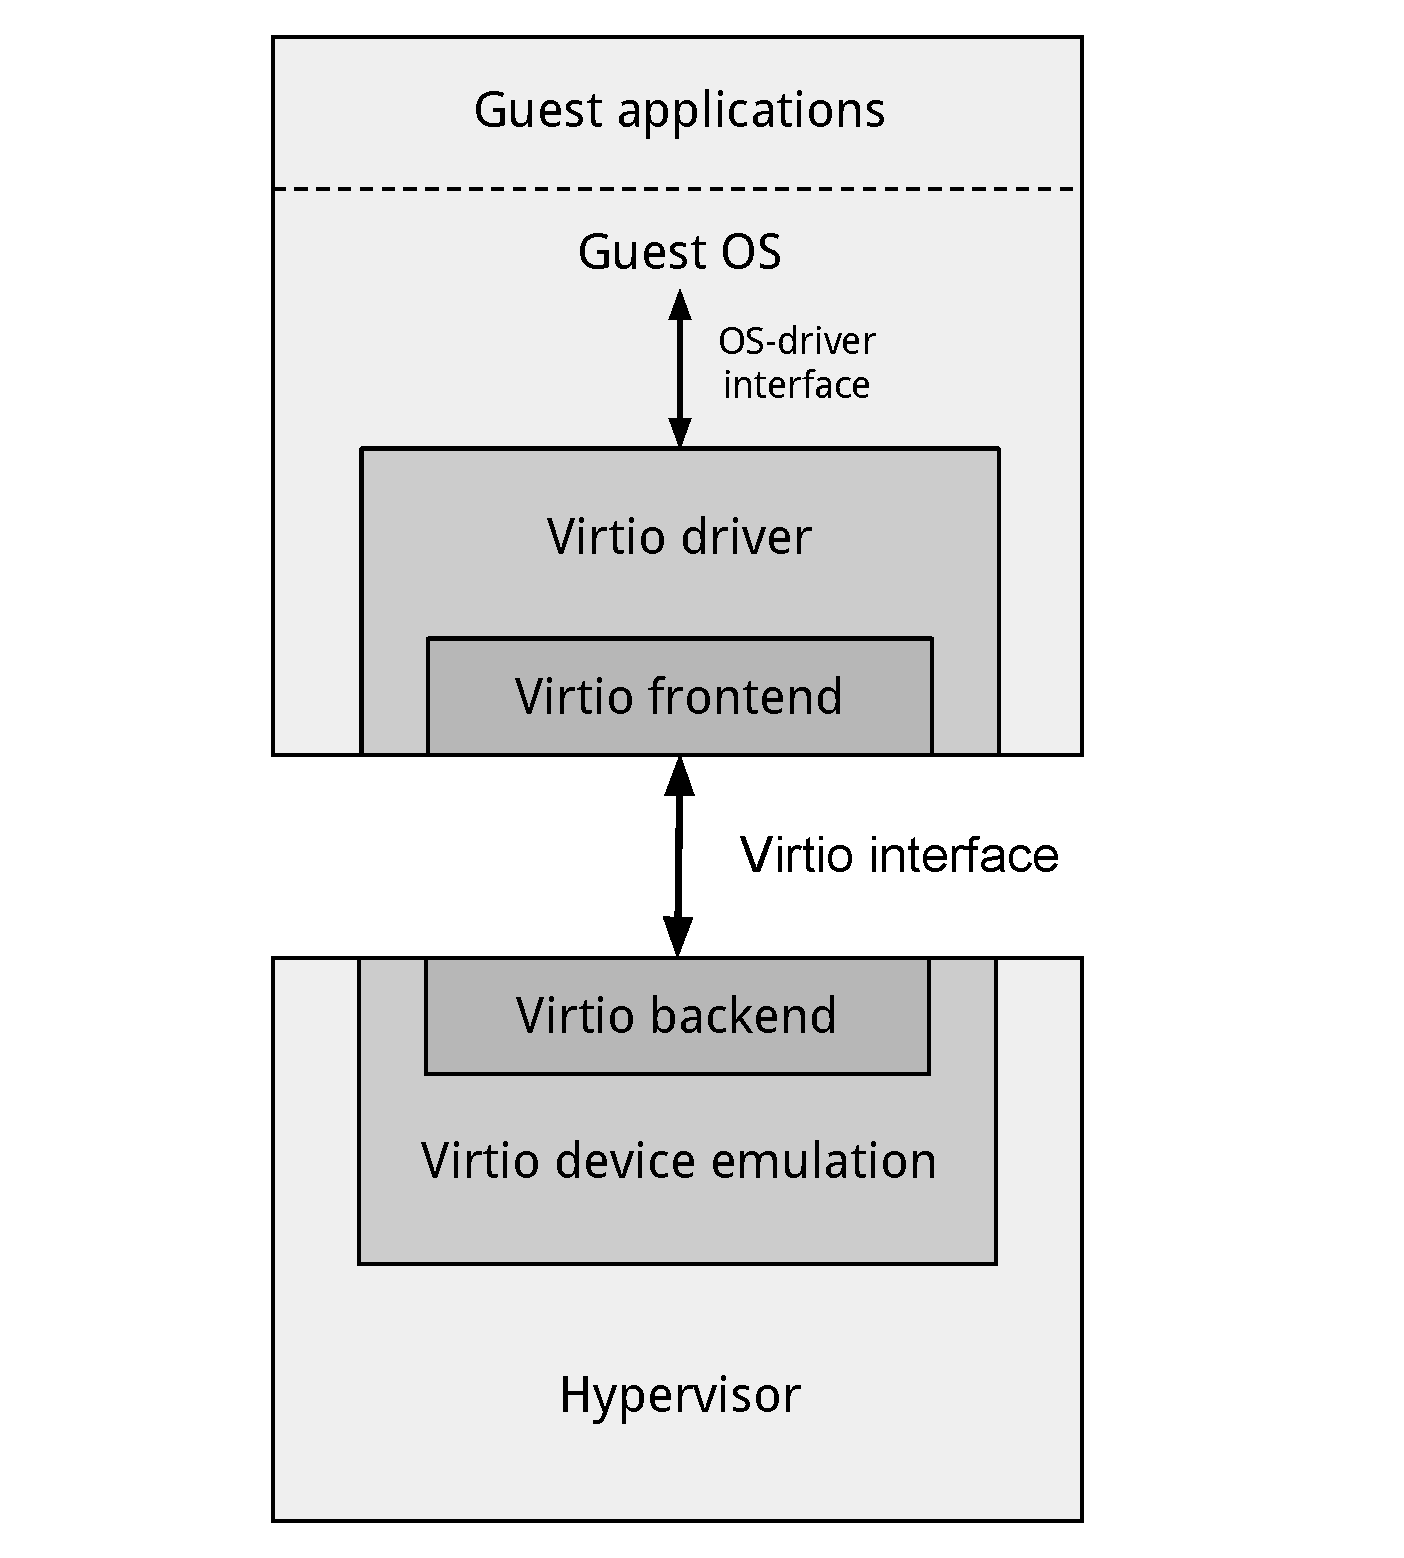
\includegraphics[scale = 0.45]{virtio.pdf}
\caption{A guest and its hypervisor communicate through the Virtio interface. The Virtio backend and Virtio frontend, together, implement
	the Virtio interface.}
\label{fig:virtio}
\end{figure}

As we can see from figure \ref{fig:virtio}, the Virtio interface is implemented through a \emph{virtio frontend} in the guest OS, and a 
\emph{virtio backend} in the hypervisor.
All the virtio device drivers can share the virtio frontend code. The task of a virtio driver is therefore to
convert the OS representation of the data to exchange (e.g. a network packet) into the standard virtio data format, or the other way
around. All the virtio device emulators (e.g. the QEMU frontend for each virtio device) can share the virtio backend code. The task
of a virtio device emulator is therefore to convert the virtio representation of the data to exchange into the hypervisor specific
representation (e.g. a buffer containg an ethernet frame), or the other way around. In this way, the guest OS and the hypervisor can
communicate through the virtio infrastructure using an efficient and general mechanism.

\vspace{0.5cm}

The organization illustrated in figure \ref{fig:virtio} is actually similar to the one used for real device emulation (e.g. e1000 
emulation). However the Virtio interface is explicitely designed for efficient communication between driver and hypervisor,
while this is not true for real device hardware/software interfaces.

\vspace{0.5cm}

In order to estabilish an efficient communication channel, the Virtio interface implementation uses MMIO accesses and interrupts only
to notify the other peer, and never to exchange data information. Whatever data exchange is done through shared memory.


\subsection{Virtual queues}
\label{sec:virtqueue}
Central to the Virtio interface is the \emph{virtual queue} abstraction, a queue that connects a virtio frontend to a virtio backend.
A virtual queue is simply a queue into which buffers are posted by the guest driver for consumption by the hypervisor: In this way
the two peers can exchange data.
A virtual queue can be used to exchange data in both directions: Therefore the posted buffers can be used both for output and for input 
operations. Drivers can use zero, one or more queues, depending on their needs. For example, the virtio network device uses two virtual
queues (one for receive and one for transmit), while the virtio block device uses only one.
The buffers used to exchange data are represented in Virtio using scatter-gather lists\footnote{Each
element in the list represents the guest physical address and the length of a physical contiguous chunk of memory.}. With a single operation
a virtio frontend can send a scatter-gather list to a virtio backend. A single scatter-gather list can specify both input and output 
requests. For example, the guest may send to the hypervisor a SG list containing three buffers: An output buffer that specifies a 
command and two input buffer that will be filled by the hypervisor with the response\footnote{This example could be valid for a virtio
disk.}.

\vspace{0.5cm}

In more detail, when the guest wants to make requests to the hypervisor through a virtual queue, it invokes the \texttt{add\_buf} method
on the virtual queue object, passing a SG list and a non-NULL token which is returned when the SG list has been consumed. As we have seen 
previously, a single SG list can be used to pass many output buffers (e.g. network packets to send) and many input buffers (e.g. memory 
buffers where the hypervisor can store received network packets). The method returns the amount of space left in the queue, so that 
the guest can stop adding new buffers when the queue is full.
The \texttt{add\_buf} method doesn't notify the hypervisor about the new requests, but only inserts the new buffer in the virtual queue.
When a virtio driver wants to notify the hypervisor, it has to call the \texttt{kick} method. Of course
the driver should kick the hypervisor only when necessary, and try to add as many buffers as possible before \emph{kicking} the hypervisor.

When the hypervisor is notified, it extracts (pops) an SG list from the virtual queue and process the request, maybe asynchronously.
When the processing is done, the hypervisor returns the used SG list to the virtual queue.
The guest can poll for the request completion through the \texttt{get\_buf} function. This function is not blocking and returns NULL if 
there are no returned used SG lists, or returns the token associated to a SG list that has been consumed. Only when
\texttt{get\_buf} is invoked the queue space used by a previous \texttt{add\_buf} is freed.

The whole process is depicted in figure \ref{fig:virtqueue}.

\begin{figure}[bt]
\centering
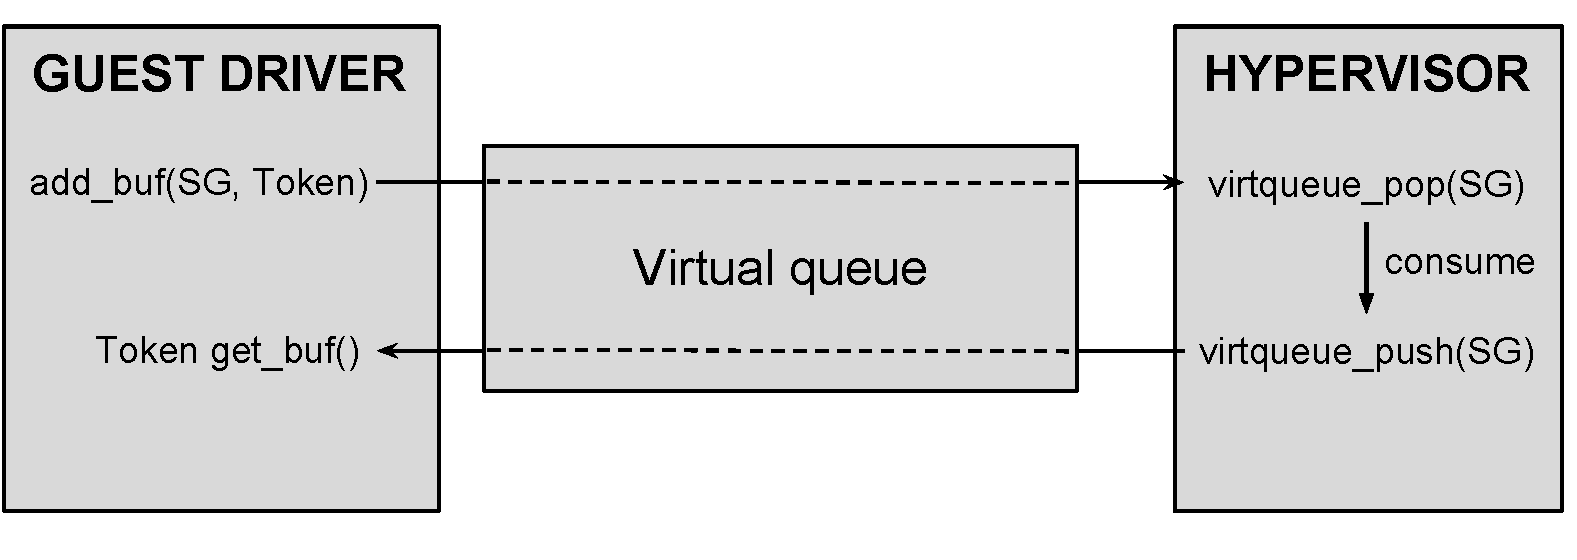
\includegraphics[scale = 0.48]{virtqueue.pdf}
\caption{Virtual queue operations. The guest adds new buffers (represented as scatter-gather lists) to the virtual queue. The hypervisor
	consumes (uses) those buffers and returns them to the virtual queue. Tokens are used by the guest to identify buffers.}
\label{fig:virtqueue}
\end{figure}

\vspace{0.5cm}

In order to avoid busy waiting, the driver can provide a callback function to a virtual queue. This callback will be invoked when the
hypervisor notifies that new used buffers have been returned. Since hypervisor notifications are generally expensive (in QEMU-KVM they are 
implemented as interrupts to the guest, so they are extremely expensive), the driver should implement strategies aimed at mitigating the
notification rate (e.g. with NAPI). In order to do that, the driver can enable or disable callbacks (e.g. enable/disable interrupts) 
invoking the \texttt{enable\_cb} or \texttt{disable\_cb} methods on the virtual queue. The \texttt{disable\_cb} is actually only a hint,
there is no guarantee that the callback will not still be called right after, since this would require expensive synchronization: It is
just an optimization to reduce unnecessary notifications.
The callback function can call the \texttt{get\_buf} so that it can process the used buffers.

\vspace{0.5cm}

In a similar way, the hypervisor can enable/disable guest notifications (kicks)\footnote{e.g. In our work environment this are
implemented as guest MMIO accesses.}, since also this notifications are very expensive. When guest notifications are disabled,
the \texttt{kick} method has no effect.


\subsection{The virtio ring transport mechanism}
In the current implementation, the virtual queues are implemented as \emph{rings}, similarly to what happens with network adapters (see
section \ref{sec:e1000-interface}). The Virtio interface hides the rings, so that we could use a different implementation as
long as both virtio frontend and virtio backend use the same transport mechanism.
Since a virtio ring must be a very general and flexible mechanism for transporting buffers, it is also quite complex, or at least more
complex than needed for and efficient paravirtualized network device.

\vspace{0.5cm}

A virtio ring consists of three parts: the descriptor array where the guest chains together length/address pairs (taken from a guest-provided
SG list), the \emph{available} ring where the guest indicates what descriptors chains are ready for use, and the \emph{used} ring where the
host indicates which descriptors chains it has used. Each descriptor contains the guest-physical address of the buffer, its length, an 
optional \texttt{next} index for buffer chaining, and two flags: one to indicate whether the next field is valid and one controlling 
whether the buffer is read-only or write-only. This allows a buffer chain to contain both readable and writable parts (this is 
useful for implementing a block device).

The available ring consists of a free-running index (the \emph{avail} index)\footnote{The ring index is a 16 bit unsigned integer, 
which is always incremented and is intended to overflow.}, an interrupt suppression flag, and an array of indices into the descriptor array 
where each index references the head of a descriptor chain. As we can see, the available ring is separated from the descriptor array, 
adding another level of indirection: The avail index references an entry of the avail ring and this entry references an entry of the
descriptor array (an head of a descriptor chain).
This separation of the descriptor array from the available ring is due to the asynchronous nature of the virtqueue. In fact the hypervisor
extracts the chains in the same order in which they have been inserted, but may process them in a different order and/or asynchronously.
In this case some chains could require more time than others, and so the available ring could circle many times with fast-serviced
chains while slow descriptors might still await completion (once again this is useful for block device implementation).
The interrupt suppression flag is set when the virtio driver invokes the \texttt{disable\_cb} and is suppressed when the
\texttt{enable\_cb} is invoked. In this way the guest can implement a mitigation strategy for hypervisor notifications (see section 
\ref{sec:virtqueue}).

The used ring has the same structure of the the available ring, but is written by the host as descriptor chains are consumed. Moreover,
the each entry of used ring contains not only an index in the descriptor array, but also a \texttt{len} field which is used for input
buffers: When an input buffer has been used, the hypervisor writes in this field the size of the read operation which has been done on 
the buffer itself.

The data structures are depicted in figure \ref{fig:vring}.

\begin{figure}[bt]
\centering
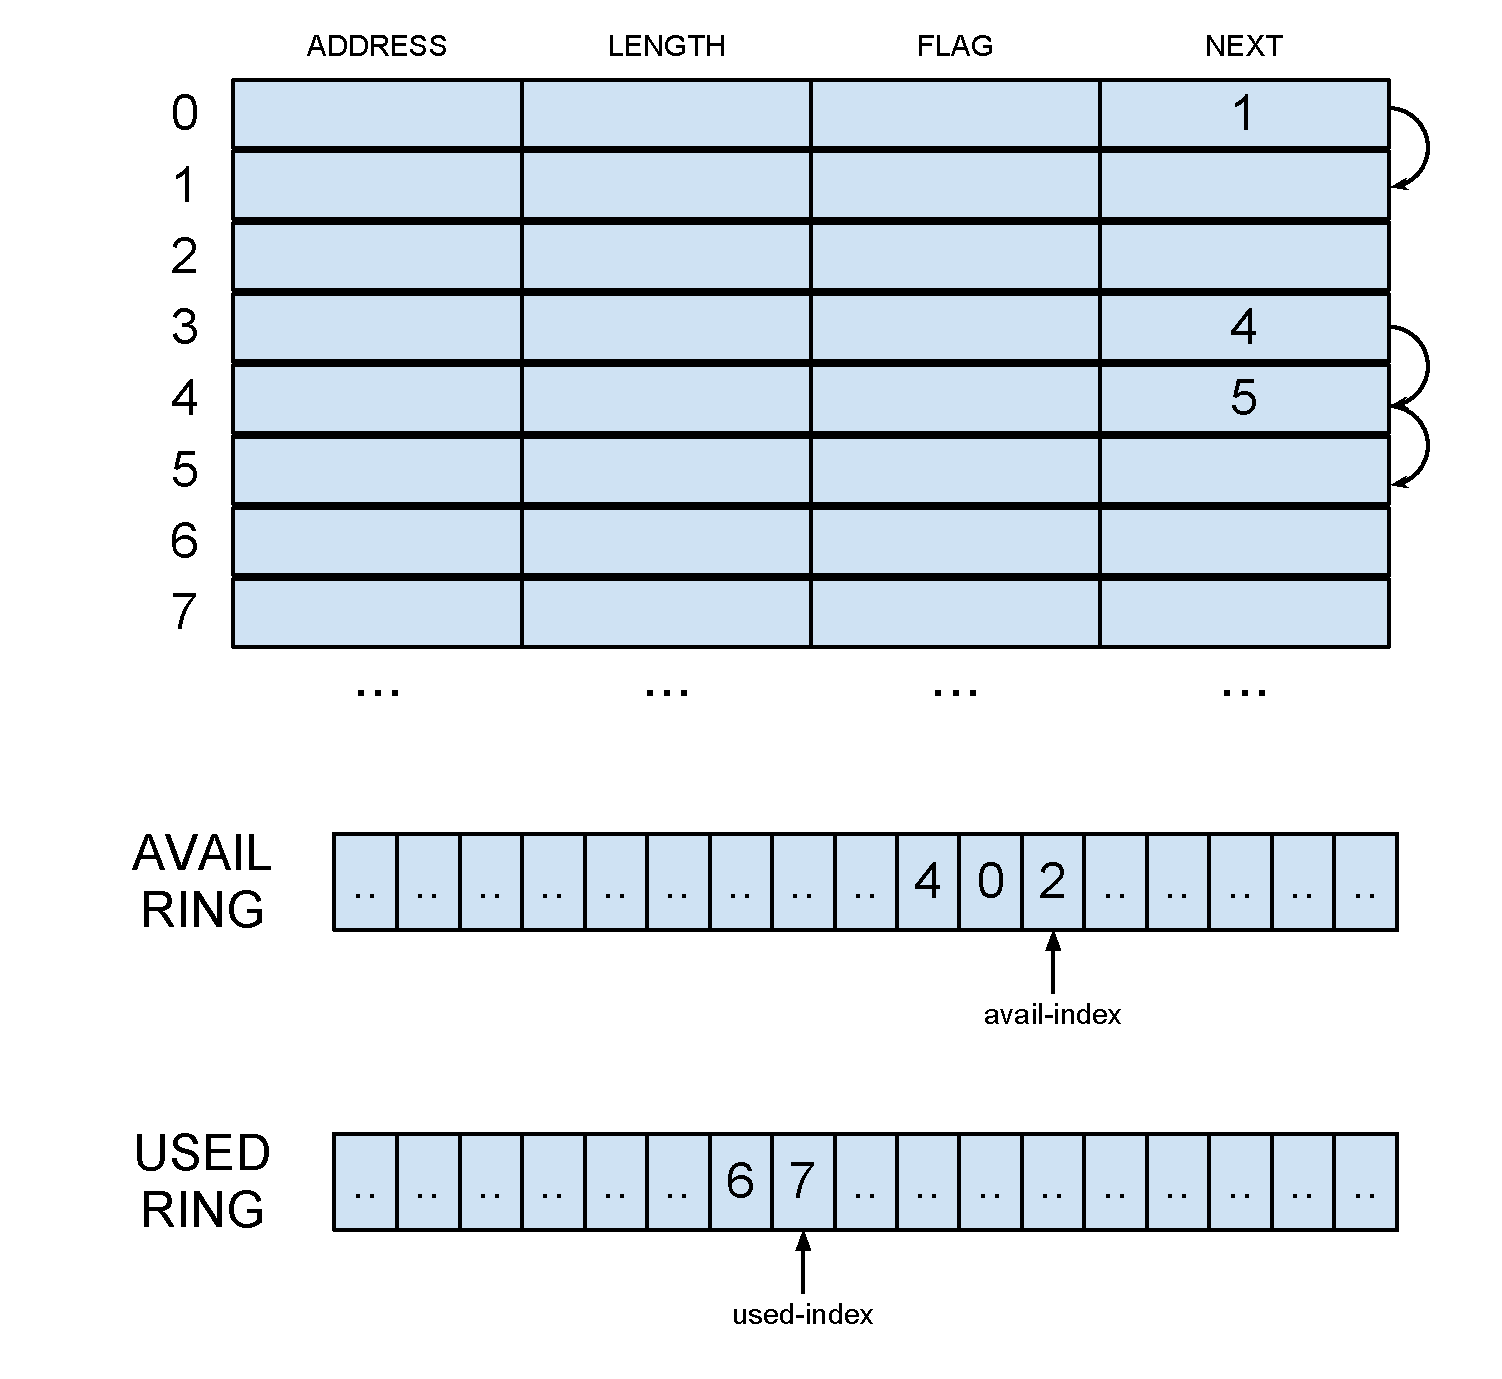
\includegraphics[scale = 0.48]{vring.pdf}
\caption{Virtio ring data structures, used to implement the Virtio interface. On the top the descriptor array is depicted as a table.
	 On the bottom the \emph{avail} ring and the \emph{used} ring.}
\label{fig:vring}
\end{figure}

\vspace{0.5cm}

Putting all together, let's describe the journey of a virtio buffer in a virtual queue. A virtio driver invokes \texttt{add\_buf} on the
virtual queue, and the provided SG list is inserted in the descriptor array, using a free entry for each element in the SG list. All this
descriptors are chained together. At this point a new entry is inserted in the avail ring, referencing the head of the chain just now
built, and the avail index is incremented.
Now the virtio driver can kick the hypervisor (if is the case), because there is a new entry in the avail ring.
When the hypervisor sees that there is work to do, it pops the new entry from the available ring, processes it, pushes the used descriptor
chain in the used ring, increments the used index and, if is the case, notifies the guest (e.g. send an interrupt). When the guest wants 
to get an used buffer, it invokes the \texttt{get\_buf} method so that it can clean or complete to process the returned buffer.


%\subsubsection{The VIRTIO\_RING\_F\_EVENT\_IDX feature}


\subsection{Minimizing notifications using Virtio}
\label{sec:virtiomin}
Let's see how we can build an Virtio driver and device emulator that try to minimize the notification rate in both directions, assuming we
are dealing with our usual work environment (QEMUKVM as VMM and Linux as guest).
As we've seen so far, in our work environment notifications are very expensive, and so minimizing them leads to big performance
improvements. Since Virtio is explicitely designed to work in a virtualized environment, it's easy to write a driver that minimizes
notifications.
We will make an abstract example where the virtio driver, using a single virtual queue, receives requests from the kernel and passes
these requests (represented as virtio buffers) to the hypervisor. The hypervisor processes these requests in a dedicated thread and returns 
the used buffers to the virtio driver. When the guest is notified by the hypervisor, the virtio driver gets the used buffers and do some
post processing. To be more precise, we would like to minimize the ratio between the average notification rate and the average request rate,
e.g. maximize the percentage of spared notifications.

\vspace{0.5cm}

\begin{figure}[bt]
\centering
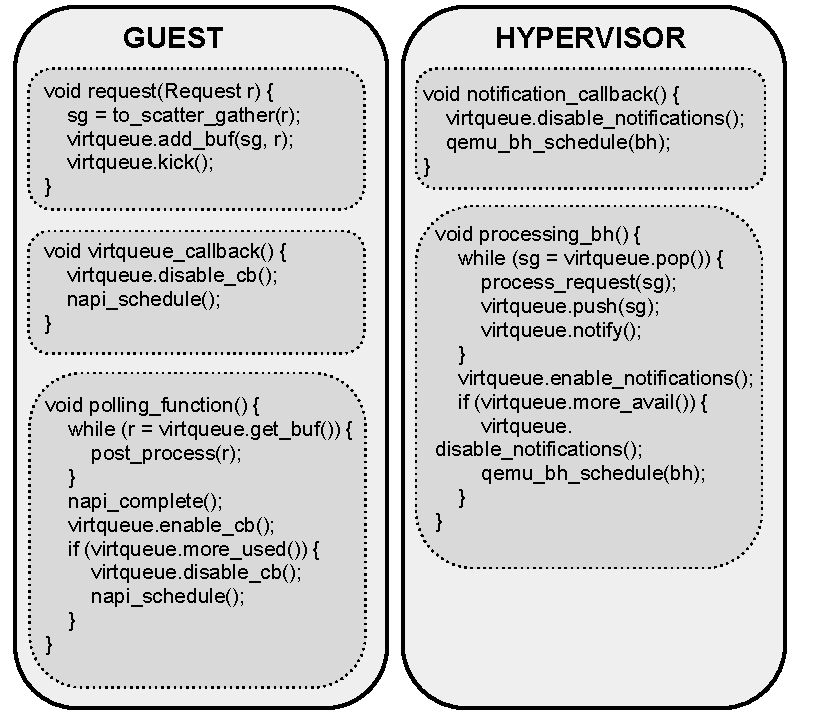
\includegraphics[scale = 1.0]{virtiocode.pdf}
\caption{Pseudocode for the virtio driver and the virtio device emulation for the example in section \ref{sec:virtiomin}.}
\label{fig:virtiocode}
\end{figure}

The pseudocode for the virtio driver and the corresponding device emulation into the hypervisor is reported in figure
\ref{fig:virtiocode}. This pseudocode skips many details, but contains all the interesting strategies to minimize notifications.
The request processing in the hypervisor is done in the IOThread, using a QEMUBH (section \ref{sec:qemuel}). The QEMUBH is scheduled
in the \texttt{notification\_callback} function, which is executed by a VCPU thread after a VMExit due to a guest notification.
As we have already seen, the guest can notify the hypervisor using the \texttt{kick} method, which turns into a real notification
(e.g. a VMExit) only if the hypervisor has the notifications enabled.
The postprocessing is done by the NAPI polling function, which runs in a dedicated thread, and is scheduled by the virtqueue callback
(\texttt{virtqueue\_callback} function). The callback is executed in interrupt context when the hypervisor notifies the guest with
an interrupt.

\vspace{0.5cm}

In conclusion, there is a dedicate worker both in the host (the QEMUBH) and in the guest (the NAPI polling function). Each worker runs
in a separate thread, so that there is parallelism. When the guest notifies the host, the host worker starts its processing and stops
only when there is no more work. When the host notifies the guest, the guest worker starts its processing and stops only when there is
no more work. Note that the processing system is symmetric: There are two symmetric \emph{producer/consumer couples} (in short PCCs). In 
the first PCC, the producer is the guest kernel which continuosly invokes \texttt{request()}, and the consumer is the QEMUBH, which 
continuously processes (comsumes) the requests. In the second PCC, the producer is the QEMUBH itself which invokes 
\texttt{virtqueue.push()} and the consumer is the NAPI polling function that does the post processing.

\vspace{0.5cm}

How are the notification minimized? Using the very same ideas introduced by NAPI (see section \ref{sec:napi}): When a notification comes,
if the notification rate is high because the incoming work request is high, we disable notifications and start polling for
requests. While there are requests to process we keep processing, keeping the notifications disabled. When there are no requests left, we
exit the working cycle and enable notifications, so that we can be notified in the future when new requests will come.
This concept is employed for both the PCCs. To be precise, after the notifications have been enabled the consumer 
checks again if there is other work to do. If true the notifications are disabled and the consumer reschedules itself. This is done because
of a race condition that we will show in the following ``Race condition analysis'' subsection.
Using this system, if the consumer is slower than the producer (see the discussion repoted in section \ref{sec:e1000-rx-g2h1vcpu}), the 
performance of the consumer/producer are very good.

\vspace{0.5cm}

Let's analyze how this system works, assuming the producer slower than the consumer in both PCCs. At the beginning notifications are 
enabled in both driver and device emulator. As the kernel invokes \texttt{request()} for the first time, the request is added to the 
virtualqueue and the kick notifies the hypervisor. Because of the
notification, \texttt{notification\_callback()} is invoked: Further guest notifications are disabled and the QEMUBH worker is
scheduled. The QEMUBH worker starts processing requests and keep doing it as the virtqueue avail ring is not empty (and because of our 
assumptions this is very unlikely to be empty). After the first request has been processed, the host successfully notifies the guest 
(\texttt{virtqueue.notify()}), and therefore \texttt{virtqueue\_callback()} is invoked: Further host notifications are disabled and the
NAPI polling function is scheduled. The polling worker starts to post-process requests and keeps doing it as the used ring is not empty 
(and it is unlikely to be so because of our assumptions). 

\vspace{0.5cm}

As we can see, this system can, in theory, work without notifications, except for the first two ones. Of course this is not realistic, also
because a consumer could be faster than a producer. For instance, the guest consumer (NAPI polling function) is often a fast one, and
so the NAPI could not moderate adequately the host notifications. In this situation, some other form of moderation is necessary to get
good performance.

Moreover, the \texttt{request()} function could implement some form of stream control and tell the kernel to stop sending requests when it
sees that the avail ring is full. If requests stop, also the two consumers stop and notification must be enabled, otherwise we couldn't
tell the kernel to restart requesting. When the guest is notified again, the kernel can restart sending request 
(causing another notification). Nevertheless, the notification rate can still be very low w.r.t. the request rate.


\subsubsection{Race condition analysis}
The consumer working cycle exits when there is no work left. Once exited, the notifications are enabled. The race exists because these
two operations, namely checking for more work and enabling notifications are not atomic. If in beetween these operation the producer
inserts more request in the virtual queue and tries to notify the consumer, the notification of this last request is not done because 
notifications are disabled. If the consumer does not double check for more work after enabling notifications, and the producer doesn't
add other requests for an hour, the last request stalls in the queue for an hour. Since the consumer double checks, however, it sees
that new requests have come while it was not polling and reschedules itself (and possibly consume the request immediately). In this
way requests cannot stall. Figure \ref{fig:race} shows an example of race.

\begin{figure}[bt]
\centering
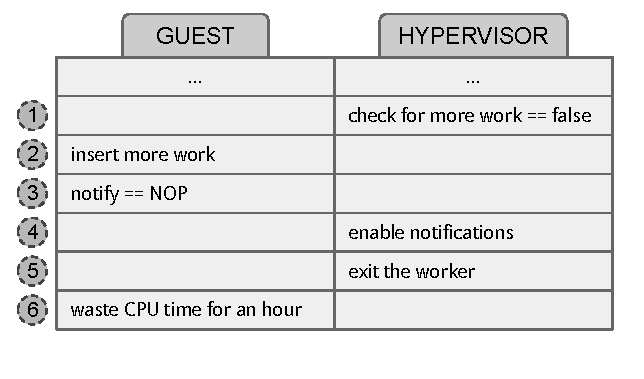
\includegraphics[scale = 1.0]{race.pdf}
\caption{Race condition between a producer and a consumer. The race condition exists because the consumer doesn't have a way to check for
	 more work and enable notifications in an atomical manner.}
\label{fig:race}
\end{figure}


\subsubsection{Other details}
In our example we've skipped many details in order to keep the pseudocode simple. However, it's important to note that both the NAPI
polling function and the QEMUBH, in their working cycle, must limit the amount of work done, otherwise they would monopolize the VCPU
thread (in the NAPI case) or the IOThread (in the QEMUBH case). For these reason the workers must count the requests processed and
exit the working cycle when the count exceeds a given amount. In the NAPI case, this amount is passed to the polling function in the
\texttt{budget} argument, whereas in the QEMUBH case we have to choose a value (e.g. 256 is a good compromise between performance and
responsiveness of the event-loop).



\section{An efficient Virtio network driver}
\label{sec:virtionet}
Using the idea presented in section \ref{sec:virtiomin} one can build a very efficient virtio network driver and network device emulator 
(\emph{virtio-net}). The driver source can be found in the linux kernel sources (drivers/net/virtio\_net.c), while the device
emulation can be found in the the QEMU source (hw/virtio-net.c).
Since a network adapter deals with two independent data streams, one for TX and one for RX, two virtual queues are employed. The virtio
block device uses just one virtual queue because the two streams are not independent, but are always request and response.

\vspace{0.5cm}

For each virtual queue, two PCCs can be defined: the \emph{direct} PCC and the \emph{inverse} PCC, depending on who is the communication
master.
On the TX path the guest is the master: in the TX direct PCC the guest produces TX avail buffers to send and the hypervisor consumes (sends)
avail buffers, while in the TX reverse PCC the hypervisor produces used buffers and the guest consumes (frees) used buffers.
On the RX path the hypervisor is the master: in the RX direct PCC the hypervisor produces (receives into) RX used buffers and the guest
consumes (receives from) RX used buffers, while in the RX reverse PCC the guest produces RX avail buffers and the hypervisor uses RX
avail buffers. This situation is depicted in figure \ref{fig:pccs}.

\begin{figure}[bt]
\centering
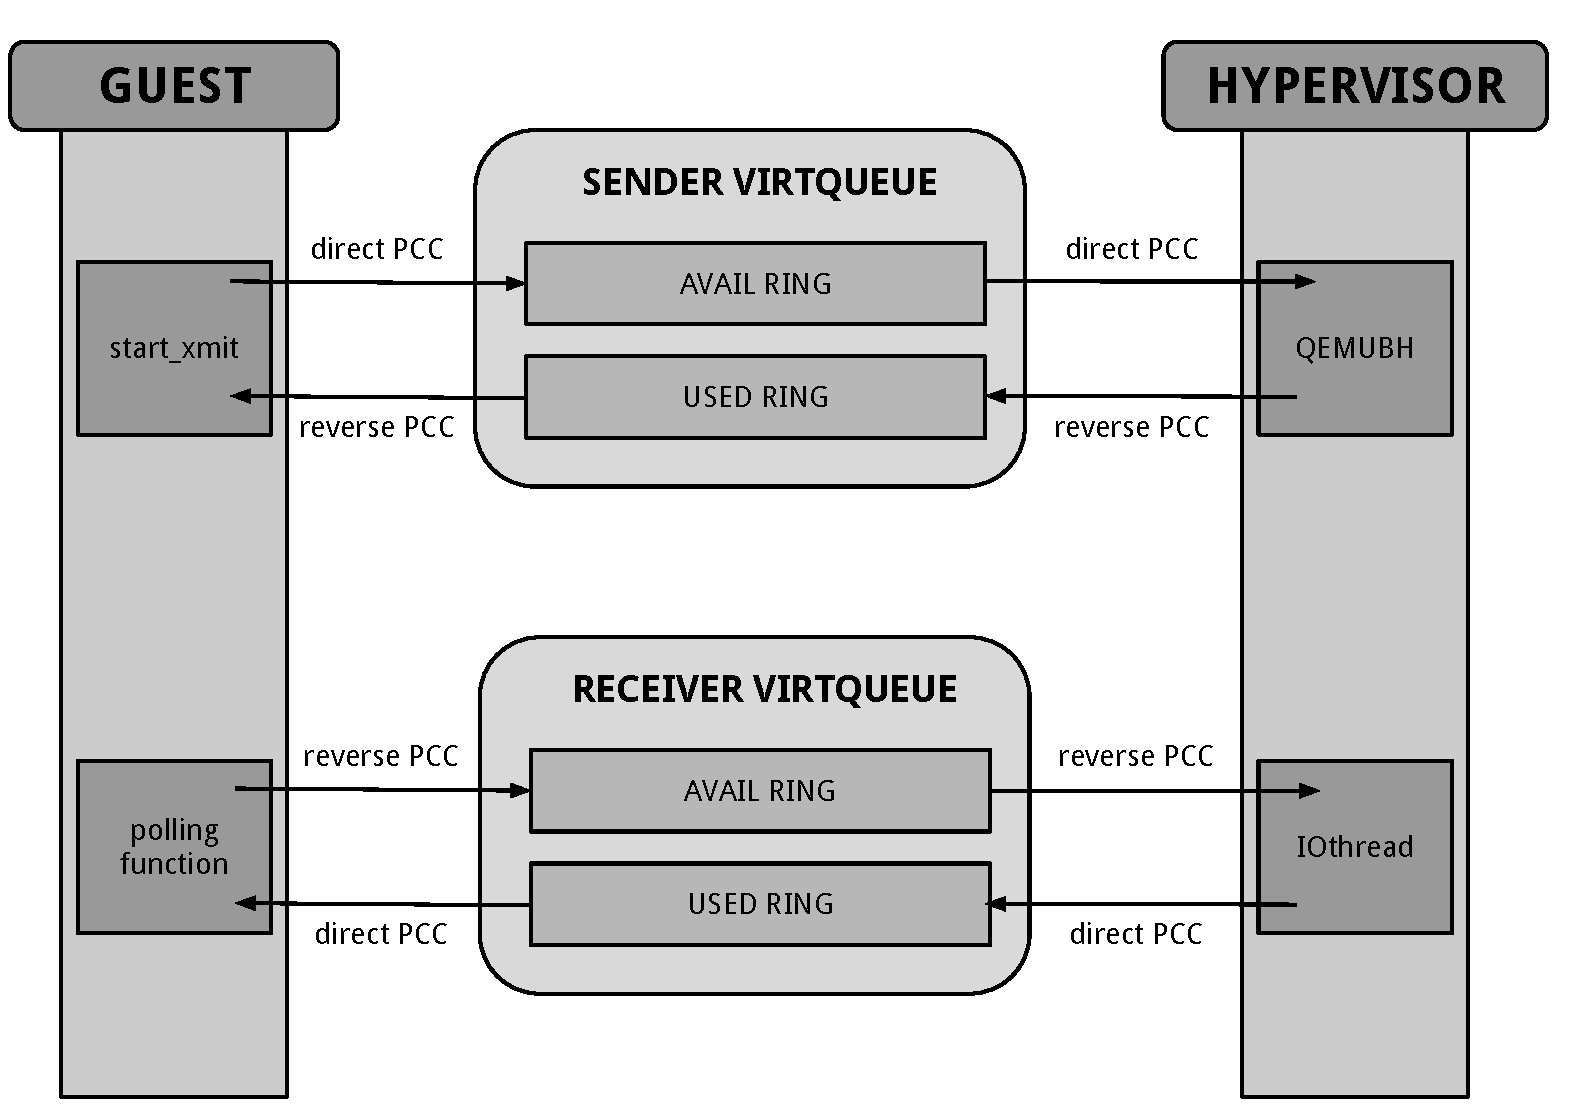
\includegraphics[scale = 0.55]{pccs.pdf}
\caption{High level scheme of the virtio-net implementation. On the top there is the sender virtual queue with its two Producer/Consumer
	 Couples (PCCs), which handle the TX path. On the bottom there is the receiver virtual queue with its PCCs, which handle the
	 RX path.}
\label{fig:pccs}
\end{figure}


\subsection{TX path}
\label{sec:virtionet-tx}
The TX path uses the sender virtual queue (\texttt{svq}), where the virtual queue callback is initially disabled on the driver side.
When the kernel invokes the \texttt{ndo\_start\_xmit} method, it does the following
\begin{enumerate}
  \item Free any pending used buffers in the used ring repeatedly calling \texttt{svq.get\_buf()}. The token returned is a pointer to a
	\texttt{sk\_buff} that was previously added to the avail ring, so that the \texttt{sk\_buff} can be freed with
	\texttt{dev\_free\_skb(skb)}.
  \item Convert the \texttt{sk\_buff} provided as argument to a SG array. The SG array will have more elements if the
	\texttt{sk\_buff} is nonlinear or just an element if linear.
  \item Invoke \texttt{svq.add\_buf(sg, skb)} to insert a new output SG in the avail ring.
  \item Invoke \texttt{svq.kick()} to notify the hypervisor.
  \item Call \texttt{skb\_orphan(skb)} so that the kernel won't wait for the \texttt{sk\_buff} to be freed and so won't invoke the
	TX watchdog.
  \item If there is no space in the virtual queue for the next send, tell the kernel to stop making new TX requests by calling
	\texttt{netif\_stop\_queue()} and invoke \texttt{svq.enable\_cb\_delayed()}\footnote{This is a variant of the \texttt{enable\_cb}
	method that delays the abilitation in the future. The variant is implented only if the Virtio EVENT\_IDX feature is set. However,
	you cannot specify how far in the future the abilitation will take place.}.
	We will be notified by the hypervisor when this pushes more used buffer to the used ring, so that we can
	call \texttt{netif\_wake\_queue()} and the kernel can make new TX requests.
	After notification are enabled we must do a double check for more used buffers otherwise we would run into the same race condition
	described in section \ref{sec:virtiomin}. If there are more used buffers, we free them (in the same way as we do at point 1) and,
	if now there is space enough for a new send, we disable the callback and tell the kernel it can restart making TX request (invoking
	\texttt{netif\_wake\_queue()}).
\end{enumerate}
Note that while the avail ring is not full (e.g. while the \texttt{add\_buf} is successful) the sender virtual queue callback is never used,
since the used buffers are cleaned at the beginning of the the \texttt{ndo\_start\_xmit} method.
However, when there is no more space, the kernel is told not to call this method anymore, and so the only way to free used buffer after that
is to use the callback.

\vspace{0.5cm}

The device emulator part of the TX path is implemented with the same scheme presented in section \ref{sec:virtiomin} (see figure
\ref{fig:virtiocode}), where the guest notification are initially enabled.
In this way the guest notification are moderated when the guest sender is faster than the QEMUBH TX processing cycle.
The TX processing is done basically calling \texttt{qemu\_sendv\_packet(sg)}\footnote{This is a simple variant of the
\texttt{qemu\_send\_packet()} function, that accepts a scatter-gather array.}, where \texttt{sg} is the SG list extracted by the avail ring.
A copy is not performed in the hypervisor, but is necessary to map the guest physical memory onto the hypervisor virtual memory, since the
virtio descriptors contains physical addresses. This mapping, however, is done internally by the \texttt{virtqueue.pop()}, so it's not
visible to the device emulator.


\subsection{RX path}
The RX path uses the receiver virtual queue (\texttt{rvq}), where the virtual queue callback is initially enabled on the driver side.
At initialization time, the driver must provide the hypervisor with some receive buffers, otherwise it cannot accept incoming
packets\footnote{We've seen the same problem with e1000 in section \ref{sec:rxdriver}.}. In other words, the driver has to fill the avail
ring with receive buffers calling \texttt{add\_buf()} as many times as possible. A pointer to an empty \texttt{sk\_buff} is passed as
token.

\vspace{0.5cm}

On the device emulation side (virtio-net frontend), the guest notification are initially enabled.
When the hypervisor receives a packet, the network backend invokes the \texttt{virtio\_net\_receive} method, that performs the
following actions:
\begin{enumerate}
  \item If there are no receive buffers to use, enable guest notifications, so that we will be notified when more receive buffers
	are added to the avail ring. Then return 0 (the number of bytes received). When the QEMU network core sees that the virtio-net
	frontend is not able to receive the packet, it puts the received packets into an internal queue (see section \ref{sec:frontback}). 
	When the guests notification comes, the frontend invokes \texttt{qemu\_flush\_queued\_packets()}, so that the QEMU network core 
	tries again to invoke \texttt{virtio\_net\_receive} on each queued packet.
	After we enable guest notifications, we must double check for more avail buffers, otherwise the usual race condition can show up.
	
  \item Pop a receive buffer from the virtual queue (\texttt{rvq.pop(sg)}).
  
  \item Copy to this receive buffer the ethernet frame passed to \texttt{virtio\_net\_receive}.
  
  \item Pushes the used buffer to the used ring. To be precise, the push operation is not performed with the \texttt{push} method, 
	but in two (or more) splitted calls. Firstly the \texttt{fill} method is called to put an used SG list in the ring without
	updating the user ring index, and then the \texttt{flush} method is called to update the used ring index. The reason for this
	is that in general we need more avail SG lists (and so more \texttt{pop}) for a single ethernet frame. Since we don't want to
	expose an used index that corrispond to a incomplete ethernet frame we can update the used index only when the received packets
	is completely in the used ring.
	
  \item Notify the guest with \texttt{rvq.notify()}.
\end{enumerate}

The driver part of the RX path is implemented with the same scheme presented in section \ref{sec:virtiomin}. The NAPI polling function is
scheduled by
the receiver virtual queue callback, which also disable further callbacks. The polling function polls for used receive buffers calling
\texttt{rvq.get\_buf()}, that returns the \texttt{sk\_buff} token. Each used buffer is processed by the \texttt{receive\_buf()} function,
which invokes the \texttt{netif\_receive\_skb()} as last operation.
When the working cycle exits, it means that the NAPI budget is over or that no more used buffer are ready.
At this point the polling function has made room in the avail ring and so refills it with new receive buffers\footnote{Observe that the
receive buffer management is very similar to the one employed by e1000.}.

After that the callbacks are enabled and the usual double check performed (with callbacks disabling and NAPI rescheduling if there are
more used buffers).


\subsection{Other details}
In this section we've outlined the most important details about \emph{virtio-net} implementation. However, we have skipped some details
such as out-of-memory (OOM) managment, and receive buffer allocation/deallocation and processing.
In fact three types of receive buffers can be used: \emph{small} buffers, \emph{big} buffers and \emph{mergeable} buffers. For further
information refer to the source code.

\vspace{0.5cm}

Another important feature is the use of TSO/GSO\footnote{Generic Segmentation Offload is a network driver feature that extends the TSO
concept to other protocols, such as UDP.} kernel support (introduced in section \ref{sec:e1000-hardware}), that allows to transmit
and receive very big packets (up to about 64KB). These features lead to huge improvements in TCP throughput with reference to a case in
which TSO/GSO packets are not used.


\subsection{Performance analysis}
In this section we will preform the same experiments presented in section \ref{sec:e1000perf}, so that we can compare the result with
the e1000 performance (patched or unpatched).

\subsubsection{TX performance}
\label{sec:virtionet-perf-tx}
The results in 1-VCPU case are shown in table \ref{tab:virtionet-tx-g2h1vcpu}. We can see that the interrupt rate is very low and the
performance is good ($\sim 160$ Kpps). At the same time, the TX notification rate is almost zero. 

\begin{table}
\begin{center}
\begin{tabular}{lrrl}
\toprule
\textbf{Virtio-net} & \textbf{1-VCPU} & \textbf{2-VCPUs} & \\
\midrule
Interrupt rate & 0.822 & 0.8 & KHz\\
TX packet rate & 158.1 & 154.8 & Kpps\\
TX bitrate & 130.3 & 127.6 & Mbps\\
TX notifications & 0.007 & 0.007 & Mbps\\
\bottomrule
\\
\toprule
\textbf{Paravirtualized e1000} & \textbf{1-VCPU} & \textbf{2-VCPUs} & \\
\midrule
Interrupt rate & 0.37 & 0.58 & KHz\\
TX packet rate & 183.4 & 182.9 & Kpps\\
TX bitrate & 135.1 & 133.1 & Mbps\\
TX notifications rate & 0.4 & 0.34 & KHz\\
MMIO write rate & 1.2 & 1.4 & KHz\\
MMIO read rate & 0.4 & 0.55 & KHz\\
\bottomrule
\end{tabular}
\end{center}
\caption{Guest to host statistics with paravirtualized solutions. The table on the top shows virtio-net performance, while the table on
	 the bottom shows paravirtualized e1000 performance. Each table reports a set of measurements for the 1-VCPU case and one for
	 the 2-VCPUs case.}
\label{tab:virtionet-tx-g2h1vcpu}
\end{table}

What happens here is that the producer (the guest) is faster than the consumer (the hypervisor) in the TX direct PCC: This is why the 
hypervisor (almost) never needs to exit from its working cycle and so (almost) never enables guest notifications.

\vspace{0.5cm}

Since the guest is faster, the sender avail ring
should be always close to full: As soon as the hypervisor consumes some avail buffers, the guest should replenish the avail ring, tell the 
kernel to stop sending packets, and enable interrupts. In the TX reverse PCC, in other words, the consumer (the guest) is faster than the
producer (the hypervisor).
In this scenario, therfore, the interrupt rate should be very high, because the system would
enter in a permanent \emph{almost-full} state:
\begin{enumerate}
  \item The sender queue avail ring has space for only one (or a very few) packet, therefore rapidly replenishes the ring and enables the
	interrupts.
  \item As soon as the hypervisor processes the next TX packet (making room in the queue), it notifies the guest. The cycle go on from
	point 1.
\end{enumerate}
In this situation we should have nearly one interrupt per packet, and so bad performance. However, from table 
\ref{tab:virtionet-tx-g2h1vcpu} we don't see this circumstance because of the way the interrupts are enabled. As we have seen in 
section \ref{sec:virtionet-tx}, the \texttt{enable\_cb\_delayed} method is used in place of \texttt{enable\_cb}. In this way the interrupts
are enabled after a while, and not immediately. In the current implementation, the interrupt are enabled when the hypervisor has processed
$\frac{3}{4}$ of the pending packets in the queue\footnote{In our case the queue is full of pending packets.}. Therefore when an interrupt
comes, 75\% of the queue is empty, and not just one packet. In other words, the system enters a state in which the guest is notified every
192 packets\footnote{The current default size for a virtual queue is 256, and so $256 \cdot 0.75 = 192$.}, and still the queue is never
empty (so the hypervisor never stops) because the guest is fast to replenish the queue. In conclusion we should expect an interrupt rate of
$\frac{158.115 Kpps}{192} = 0.823$ KHz, which is exactly what we have in the table.

\vspace{0.5cm}

Although not implemented with timers, the \texttt{enable\_cb\_delayed} method is just a different \emph{incomplete} form of interrupt 
moderation.
It is used to moderate the notification rate within a PCC where the consumer is faster than the producer: In our case
the producer is the hypervisor, which produces used buffers, and the consumer is the driver, which consumes (free) used buffers.
In order to see the mitigation effects, we have tried to run the same experiment with a modified virtio-net driver, where \texttt{enable\_cb}
is used in place of \texttt{enable\_cb\_delayed}. The results are shown in table \ref{tab:virtionet-tx-nomit-g2h1vcpu}.

\begin{table}
\begin{center}
\begin{tabular}{lrl}
\toprule
\textbf{Interrupt rate} & 108.4 & KHz\\
\textbf{TX packet rate} & 110.4 & Kpps\\
\textbf{TX bitrate} & 91.0 & Mbps\\
\textbf{TX notifications} & 0.007 & Mbps\\
\bottomrule
\end{tabular}
\end{center}
\caption{Guest to host statistics with 1 VCPU per guest, when the \texttt{enable\_cb\_delayed} method is not implemented}
\label{tab:virtionet-tx-nomit-g2h1vcpu}
\end{table}

As we can see, here the situation is exactly the one we described previously (the almost-full state), with an interrupt for each TX packet.
The TX packet rate oscillates between 80 Kpps and 150 Kpps, the system is very unstable and has a very low responsiveness: Interrupt
mitigation was definitely required in this case.

\vspace{0.5cm}

It's very important to observe that you cannot always use this form of mitigation, because of its incompleteness: there is not a 
mechanism to force timely notification of pending events. Even worse, it can be the case that a pending event stalls forever in a 
queue.
In our case, the TX reverse PCC, there is not such a problem, for two reasons:
\begin{itemize}
  \item On the TX path, the comunication \emph{master} is the guest, and so when it calls \texttt{enable\_cb\_delayed()} we are sure
	that the pending TX buffers will be processed by the \emph{slave} (the hypervisor) as soon as possible, and so the interrupt
	will be sent for sure, e.g. the pending events cannot stall.
	
  \item Considering the way the TX path is implemented (see section \ref{sec:virtionet-tx}), we don't care about having used TX buffers
	freed as soon as possible, since they are basically freed when needed.
\end{itemize}
In the RX path we are not so lucky (see the next subsection).

\vspace{0.5cm}

The results for the 2-VCPU test case are shown in table \ref{tab:virtionet-tx-g2h1vcpu}, and are very similar to results for 1-VCPU case,
since there is no significant work that can be done in parallel.


\subsubsection{RX performance}
\label{sec:virtionet-perf-rx}
The measured critical rate is about 110 Kpps, which is not very high if compared with what we get with e1000 (adding the mitigation patch).
The collected statistics are shown in table \ref{tab:virtionet-rx-g2h1vcpu}.

\begin{table}
\begin{center}
\begin{tabular}{lrrl}
\toprule
\textbf{Virtio-net} & \textbf{1-VCPU} & \textbf{2-VCPUs} & \\
\midrule
Interrupt rate & 57.6 & 43.5 & KHz\\
RX packet rate & 103.0 & 100.1 & Kpps\\
RX stream & 127.6 & 124.0 & Mbps\\
RX notification & 0.007 & 0.004 & Mbps\\
\bottomrule
\\
\toprule
\textbf{Paravirtualized e1000} & \textbf{1-VCPU} & \textbf{2-VCPUs} & \\
\midrule
Interrupt rate & 3.8 & 3.7 & KHz\\
RX packet rate & 317.3 & 315.4 & Kpps\\
RX bitrate & 231.0 & 229.6 & Mbps\\
RX notifications & 0.001 & 0.002 & Mbps\\
MMIO write rate & 7.5 & 7.4 & KHz\\
MMIO read rate & 3.8 & 3.7 & KHz\\
\bottomrule
\end{tabular}
\end{center}
\caption{Host to guest statistics with paravirtualized solutions. The table on the top shows virtio-net performance, while the table on
	 the bottom shows paravirtualized e1000 performance. Each table reports a set of measurements for the 1-VCPU case and one for
	 the 2-VCPUs case.}
\label{tab:virtionet-rx-g2h1vcpu}
\end{table}

Also in this case, the reason for low performance is tied to the lack of interrupt mitigation. As we can see, the interrupt rate is
very high (57 KHz), because Virtio does not limit the interrupt rate in any way. From an high interrupt rate we can infer that in the 
RX direct PCC, the consumer (the NAPI) is faster than the producer (hypervisor): This results in only about 2
packets processed by the polling function for each interrupt.
We could add mitigation in the same way we have added it in the TX inverse PCC (see the previous subsection): Using
the \texttt{enable\_cb\_delayed} method in place of the \texttt{enable\_cb} method when exiting from the NAPI working cycle.
However, this simply cannot be done:
\begin{itemize}
  \item On the RX path, the master is the hypervisor and so the guest (the slave), when calling
	\texttt{enable\_cb\_delayed()}, cannot know when the next packet will be received by the hypervisor, and therefore cannot know
	when a total of 192 packets will be received. Since the Virtio mitigation is incomplete, up to 191 RX packets could stall
	in the used ring. Of course, this is not acceptable.
  \item Latency is affected negatively by the mitigation in this case.
\end{itemize}
A complete form of mitigation is here the only solution, but this has not been implemented yet.

\vspace{0.5cm}

On the RX reverse PCC the consumer (hypervisor) is slower than the producer (guest) and consequently the RX notification rate is
very good (about zero notifications).

\vspace{0.5cm}

The measured results for the 2-VCPU case are shown in table \ref{tab:virtionet-rx-g2h1vcpu}. There is not a substantial difference with
the 1-VCPU case, because there is not enough parallelism in the guest to exploit.



\section{Porting paravirtualization to e1000}
\label{sec:e1000-paravirt}
In the previous sections we've seen how is possible to get good performance using a paravirtualized I/O solution. Virtio drivers are
efficient because the only make use MMIO accesses and interrupts to notify the other peer of a virtual queue, and exchange data and
metadata through shared memory.
However, the Virtio interface must also be general enough to support different kind of devices and is not specifically tailored to the
network device world: Most of the complications come from the need of a paravirtualized disk device. As an example, a network driver
doesn't need two rings (avail and used) for each virtual queue, and doesn't even need to separate the ring from the descriptor table. The
descriptor table and two indices in that table would have been enough.
Moreover, a complete mitigation scheme is not implemented, and this is a limitation in same situations (see section
\ref{sec:virtionet-perf-rx}, RX performance),
Lastly, the Virtio solution requires a completely new set of device drivers/emulators, which is a greater effort than modifying
an existing device driver/emulator.

\vspace{0.5cm}

In this section we will see how is possible to extend the e1000 interface in order to adopt the paravirtualization paradigm.
As usual, we will try to minimize the modifications to the existing code, so that the proposed patch can be easy to test and mantain.


\subsection{Asynchronous TX Processing}
\label{sec:e1000-par-async}
In the e1000 emulation we've seen so far, the TX processing is done by a VCPU thread (section \ref{sec:e1000txemu}).
A better solution however, is to employ the processing/notification scheme presented in section \ref{sec:virtiomin} (e.g. NAPI-like 
moderation), in which the hypervisor processing is done asynchronously using a QEMUBH.
In this way the TX processing is executed by the IOThread in parallel to the VCPUs.


\subsection{Communication Status Block}
In order to implement an efficient communication scheme we have to remove, where possible, MMIO accesses that exchange data, leaving only
accesses that implement guest notifications to the hypervisor.
As an example, writes to TDT and RDT registers are used for two functions:
\begin{enumerate}
  \item (notify) Notify the hypervisor that there is something new to process (new Tx descriptors to process or new Rx descriptors to use).
  \item (status) Tell the hypervisor which descriptors have just been added.
\end{enumerate}
A notification (1), however, is not always necessary\footnote{For example, it's not necessary if the other peer is in its working cycle.}, 
while status information exchange (2) is always desirable, so that the other peer is always updated and it's less likely to exit from its
working cycle.
It would then be better to split these functions: TDT/RDT writes should be used only for notifications, while status exchange can be done
using shared memory. For these reasons a dedicate block of shared memory, called \emph{Communication Status Block} (CSB), has been allocated
in the guest memory. The CSB is a set of 32-bits words that are used to exchange information about the status of the communication without
VMExits.

\vspace{0.5cm}

The CSB contains the following words:
\begin{itemize}
  \item TXSNTS (Tx Software Next To Send): is synchronized with the \texttt{tx\_next\_to\_use} variable (when in a coherent state). In 
	short, where the \texttt{ndo\_start\_xmit} starts to insert new TX descriptors in the TX ring. It is used to replace the status
	information function of the TDT register.
	
  \item TXHNTS (Tx Hardware Next To Send): is synchronized with the TDH register. In short, where the hardware takes the next TX descriptor
	to process.
	
  \item TXSNTC (Tx Software Next To Clean): is synchronized with the \texttt{tx\_next\_to\_clean} variable. In short, where the TX interrupt
	routine takes the next used TX descriptor to clean.
	
  \item RXSNTP (Rx Software Next To Prepare): is synchronized with the \texttt{rx\_next\_to\_use} variable. In short, where the driver
	adds new RX descriptors to use for reiceving new frames.
	
  \item RXHNTR (Rx Hardware Next To Receive): is synchronized with the RDH register. In short, where the hardware takes the next RX
	descriptor to use for an incoming frame.
	
  \item RXSNTR (Rx Software Next To Receive): is synchronized with the \texttt{rx\_next\_to\_clean} variable. In short, where the RX 
	interrupt routine takes the next used RX descriptor to push the received frame to the network stack.
	
  \item TXNTFY (Tx Notify Flag): Set/Cleared by the hardware to enable/disable TX notifications. At the end of the
	\texttt{ndo\_start\_xmit} method, the driver always updates TXSNTS, and updates also TDT only if TXNTFY is set.
	
  \item RXNTFY (Rx Notify Flag): Set/Cleared by the hardware to enable/disable RX notifications. After adding new RX
	descriptors in the ring, the driver always updates RXSNTP, and updates also RDT only if RXNTFY is set.
\end{itemize}

Some words (TXSNTS, TXSNTC, RXSNTP and RXSNTR) are always written by the software (the driver) and read by the hardware (the device 
emulator).
The other words (TXHNTS, RXHNTR, TXNTFY and RXNTFY) are always written by the hardware and read by the software.

\vspace{0.5cm}

How we can see, these variables capture in each moment the status of the communication (both RX and TX). Most of them are just shadow
copies of registers (TXHNTS and RXHNTR) or shadow copies of existing driver variables (TXSNTS, TXSNTC, RXSNTP and RXSNTR), therefore
nothing new so far. Shadow copies of registers are useful because the driver can read them without a VMExit. Shadow copies of existing
variables are useful only for technical reasons: they allow us to have all the interesting variables in a contiguous chunk of physical 
memory so that the driver can to tell the hardware only the CSB physical address. Otherwise the driver should tell the hardware a different
physical address for each interesting variable\footnote{In the existing e1000 driver the memory for these variables is not allocated all
together, so the driver data memory is not necessarily contiguous.}.

\vspace{0.5cm}

On the other end, TXNTFY and RXNTFY are something new. These are used by the hardware to disable TDT writes and RDT writes when
these are not necessary. As we have outlined in section \ref{sec:e1000-par-async}, the idea is to implement the usual
producer/consumer scheme (NAPI-like moderation), which requires a method for the consumer to disable producer notifications.

\vspace{0.5cm}

Similarly to what happens to the other shared memory structures (e.g. TX/RX rings), the hardware must be told where the CSB has been
allocated in the guest physical memory. For these reason, two 32-bit registers, CSBBAH (CSB Base Address High) and CSBBAL (CSB Base
Address Low) have been added to the register set. The driver must write the physical address of the CSB to these registers.


\subsection{Implementation}
This section briefly reports what changes have been added to the RX and the TX path to implement e1000 paravirtualization.
The changes are relative to the existing implementation of e1000, possibly improved with the moderation patch.
As we have already observed, interrupt moderation is very useful within PCCs in which the hypervisor is the producer, and the guest is
is faster than the hypervisor. However, the paravirtualization patch is independent on the moderation patch.
The driver batching mechanism, on the other hand, is not intended to be used jointly with paravirtualization, simply because this would not
make any sense: Since paravirtualization exports the status of the communication, there's no need to flush pending TX descriptors, we just
have to notify the hypervisor when necessary.

\vspace{0.5cm}

A new parameter, \texttt{paravirtual}, has been added to the e1000 module. The parameter value can be specified only at module loading time
and cannot be changed dynamically. When \texttt{paravirtual} is 0, the driver is the original one, and the device emulator (e1000 frontend)
behaves as usual\footnote{To keep the code simple, the CSB is always allocated even if \texttt{paravirtual} is 0.}. When 
\texttt{paravirtual} is 1, the driver allocates the CSB, initializes it, and writes its physical address to the CSBBAH and CSBBAL registers.
On the hypervisor side, the emulated e1000 hardware switches to ``paravirtual mode'' when the driver writes to the CSBBAL register and
CSBBAL/CSBBAH registers specify together a non-null address.

\vspace{0.5cm}

At initialization time, the CSB words are set to 0, except for TXNTFY and RXNTFY that are initialized to 1.


\subsubsection{Changes in the TX path}
At the end of the \texttt{ndo\_start\_xmit} method in the e1000 original driver, where the TDT would be updated, we changed the
code so that TXSNTS is updated, while the TDT is updated only if TXNTFY is set.
In the TDT write handler, TXNTFY is cleared to disable further notifications and the QEMUBH is scheduled. The QEMUBH handler invokes the
\texttt{start\_xmit} function, so that the TX processing (working) cycle is entered. The working cycle can exit because we processed
too many descriptors (256 in the current implementation) or because there is no more work to do. If the working cycle has processed at least
one descriptor, the QEMUBH is rescheduled. Otherwise TXNTFY is set to 1, and the usual double check is performed. If new work is found,
TXNTFY is cleared and the QEMUBH rescheduled. If new work hasn't come yet we don't reschedule the QEMUBH.
Note that we reschedule even if just one descriptor has been processed, and not only if a full burst (256) of descriptors has been processed:
This is a form of \emph{spinning} that can be useful when dealing with fast backends, because we make the QEMUBH more likely to be
rescheduled, and so the TX notification more likely to be disabled. The spinning can work well in this case because, after rescheduling,
the QEMUBH handler is not executed immediately, but in the next event-loop iteration, so that the guest has some time to post more work 
in the queue.


\subsubsection{Changes in the RX path}
At the end of \texttt{e1000\_alloc\_rx\_buffers} in the original driver, where the RDT would be updated, we changed the code so that
RXSNTP is updated, but RDT is updated only if RXNTFY is set.
In the RDT write handler, if the RDT write actually gives some new receive buffers, RXNTFY is cleared to disable further RX notifications.
Remember that in this last case \texttt{qemu\_flush\_queued\_packets()} is called (see section \ref{sec:frontback}). 
When the hardware runs out of receive buffers, the e1000 \texttt{can\_receive} method returns 0. Before returning, however, it has to
set RXNTFY, so that when new receive buffers are put in the RX ring, a RDT write can flush the queued packets (if any).
After notifications have been enabled, as usual, a double check is performed in order to avoid race conditions.


\subsubsection{Other changes}
Since we know to be in a virtual machine environment, some more optimizations can be done.
In particular, after writing to IMS and IMC registers (see section \ref{sec:e1000-tx-g2h1vcpu}), we can avoid reading the STATUS register
to flush the previous register write, since there's no need to do so on the emulated hardware.


\subsection{Improvement analysis}
In this section we will perform the usual experiments (see section \ref{sec:e1000perf}), so that we can evaluate the performance
improvements. The e1000 module has been loaded with the following parameters:
\begin{center}
\begin{tabular}{ll}
\toprule
\textbf{Parameter} & \textbf{Value}\\
\midrule
TxIntDelay & 0\\
TxAbsIntDelay & 0\\
InterruptThrottleRate & 4000\\
batching & 0\\
paravirtual & 1\\
\bottomrule
\end{tabular}
\end{center}


\subsubsection{TX performance}
The results for 1-VCPU case are shown in table \ref{tab:virtionet-tx-g2h1vcpu}.

As we can see, performance are better with reference to the previous tests (both e1000 and Virtio). The interrupt rate is very low,
thanks to mitigation and NAPI. The TX notification are minimized because of the usual NAPI-like scheme.
Note that the total MMIO access rate is 1.611, which is about 4.35 times the interrupt rate: 3 MMIO accesses per interrupt are due
to the ICR read and IMC and IMS write, while 1.35 access per iterrupt are due to the TX notifications.

\vspace{0.5cm}

The results for the 2-VCPU test case (shown in table \ref{tab:virtionet-tx-g2h1vcpu}) are very similar.



\subsubsection{RX performance}
In the 1-VCPU case the measured critical rate is about 315 Kpps, which is the best result so far. Table \ref{tab:virtionet-rx-g2h1vcpu}
shows the statistics when the VM accepts an incoming rate of about 317 Kpps.

The very good result is due to the interrupt moderation, the NAPI, the MMIO access optimizations (avoid reading the STATUS register to
flush the register write) and the RX notification moderation.
The total MMIO access rate is 11.318 KHz, which means about $\frac{11.318 KHz}{3.774 KHz} \sim 3$ MMIO access per interrupt. These three
interrupt are the ICR read, and the IMC and IMS writes. RX notifications are essentially absent, because these notifications are enabled
only when the RX ring has not receive buffers to use, e.g. when the hypervisor start to be faster than the guest on the RX path.
In our case the incoming rate is still too low to make that situation very likely.

\vspace{0.5cm}

With 2 VPCUs the measured critical rate is also about 315 Kpps. Table \ref{tab:virtionet-rx-g2h1vcpu}
shows the statistics when the VM accepts an incoming rate of about 315 Kpps.
